\documentclass[11pt]{article}
\usepackage[margin=0.8in]{geometry}
\usepackage{amsmath,amssymb,booktabs,graphicx}
\usepackage[T1]{fontenc}
\usepackage{lmodern}
\usepackage[hidelinks]{hyperref}

\title{Magnetic Fields from Measurements}
\author{J. R. Landers}
\date{November 2026}
\hypersetup{pdftitle={Magnetic Fields from Measurements},pdfauthor={J. R. Landers}}

\newcommand{\B}{\mathbf B}
\newcommand{\x}{\mathbf x}
\newcommand{\rr}{\mathbf r}
\newcommand{\bvec}{\mathbf b}
\newcommand{\sech}{\operatorname{sech}}

\begin{document}
\maketitle

\begin{abstract}
What can a textbook equation learn from a robot crossing a room? In these
experiments, the physical representation accounts for most of the observed
gain, while intermediate Gaussian smoothing adds little.
A Gaussian kernel turns 500 indoor magnetic readings into a smooth map without
knowing any physics, whereas a sum of textbook dipole responses builds
magnetostatics directly into the model. A natural question is whether
pre-smoothing the data with the kernel helps the physical fit, or whether the
physical form does the work on its own. Fitting 100 dipoles and a uniform
background to the Gaussian map cuts held-out vector root mean square error from
8.09 to 5.22 (in the sensor's recording units), but fitting the same dipoles
directly to the raw readings achieves nearly the entire gain at 5.31.
Random-forest and boosted-stump baselines score 10.56 and 14.70, respectively,
under the same data protocol. At fixed settings, the dipole field is an exact
weighted sum of the original readings;
tracking those weights shows that even a small shift in route error can mask a
large change in how individual measurements are used. In a simulated wire
experiment where the learner must also choose the formula from a library, both
routes recover the field's proportionality to current and inverse scaling with
distance, yet direct fitting achieves the lowest mean error in all five regimes.
Together, the wire shows how readings can select a physical law without
intermediate smoothing, and the room shows exactly how a textbook field absorbs
empirical data.
\end{abstract}

\section{From an experiment to a field}

Switch on a current beside a compass and the needle turns. A field equation
gives that deflection a place in a larger account of electricity and magnetism.
In his 1865 paper, Maxwell began with the problem of reducing observed forces
to mathematical form and went on to develop a dynamical theory of the
electromagnetic field~\cite{maxwell}. The theory grew from experiment and
mathematical reasoning together. Once we have the equations, we can turn the
problem around: given readings from a particular experiment, what can they tell
us about the field that produced them?

Consider a robot crossing a room with a magnetometer. Each record along its
route pairs a planar position with three numbers giving the local magnetic
field. From those readings, a Gaussian kernel can interpolate a smooth map at
unvisited positions without invoking any physical law. Alternatively, we can
represent the field as a superposition of textbook dipole responses, which
automatically obeys the static field equations in free space. A tempting
compromise is a two-stage workflow: smooth the noisy readings with the kernel
first, then fit the physical model to the smoothed map. That raises two
concrete questions: when we fit dipoles to Gaussian predictions, how does the
textbook field inherit information from the original readings, and how much of
its accuracy comes from the physical form itself rather than the smoother?

We answer the first question by rewriting a uniform background plus 100 fitted
dipoles as an exact linear combination of the 500 raw measurements, allowing us
to inspect the influence of any single reading on any prediction. To answer the
second, we fit the same dipoles directly to the raw readings under identical
settings. Finally, a simulated current-carrying wire removes the known dipole
basis and asks how much of the field's mathematical form can be discovered from
data within a candidate library. Appendix~\ref{sec:scalar} checks the recovery
and solution of a differential law in one dimension.
The results favor the supplied physical form over intermediate smoothing in
these comparisons, while an exact identity exposes how that form uses the data.

\section{What the robot records}

The Aalto robot mapped an indoor area of roughly \(6\,\mathrm m\times6\,\mathrm m\).
Each sample records a time \(t\) in seconds since the start of the trial, a
sensor position \(\x(t)=(x(t),y(t))\) in metres, and a calibrated,
orientation-corrected magnetic vector \(\B=(B_x,B_y,B_z)^{\mathsf T}\), with
\(B_z\) vertical and \({}^{\mathsf T}\) denoting transpose.
Solin et al.\ mapped these readings with a Gaussian process on a scalar
potential~\cite{solin}; later work used the same archive to estimate field
magnitude sequentially~\cite{chang} and to stitch local Gaussian process maps
across a building~\cite{abdulraouf}. Here we predict all three field components
from position alone, using time only to order the predictions
\(\widehat{\B}(\x(t))\) along the robot's route.

\subsection{A Gaussian map from the readings}

At each of \(n\) planar training positions \(\x_i\), the robot records a
three-component vector \(\bvec_i\). A Gaussian kernel of length scale
\(\ell>0\) assigns any two positions a similarity
\(k_\ell(\x,\x')=\exp(-\|\x-\x'\|^2/(2\ell^2))\), where \(\|\cdot\|\)
is the Euclidean norm. At a query position \(\x_*\), the kernel map adds one
weighted bump per training position to the sample mean \(\overline{\B}\):
\begin{equation}
 \widehat{\B}_K(\x_*)=\overline{\B}+
 \sum_{i=1}^{n} k_\ell(\x_*,\x_i)\boldsymbol\alpha_i .
 \label{eq:gaussian_response}
\end{equation}
Here \(\boldsymbol\alpha_i\) sets the magnitude and direction of the bump
centered at \(\x_i\).

Because kernel ridge regression is linear in the measured vectors, every
prediction in Eq.~\eqref{eq:gaussian_response} is a possibly signed weighted sum of
the raw readings. To make those weights explicit, stack the training readings
into the \(n\times3\) matrix \(Y\) with rows \(\bvec_i^{\mathsf T}\), let
\(I_d\) denote the \(d\)-dimensional identity, and define the averaging row
\(m^{\mathsf T}=\mathbf1^{\mathsf T}/n\) and centering projector
\(P=\mathbf1 m^{\mathsf T}\), where \(\mathbf1\) is the \(n\)-vector of ones.
Every row of \(PY\) equals the mean field \(\overline{\B}^{\mathsf T}=m^{\mathsf T}Y\),
leaving centered readings \(Z=(I_n-P)Y\). Writing \(K\) for the \(n\times n\)
kernel matrix with entries \(K_{ai}=k_\ell(\x_a,\x_i)\) and \(k_*^{\mathsf T}\)
for the query row with entries \(k_\ell(\x_*,\x_i)\), kernel ridge regression
with effective penalty \(\rho>0\) (including numerical jitter) minimizes
\(\|K\alpha-Z\|_F^2+\rho\,\mathrm{tr}(\alpha^{\mathsf T}K\alpha)\), where
\(\|\cdot\|_F\) is the Frobenius norm and \(\mathrm{tr}\) is the trace.
Since \(K\) is positive semidefinite, solving \((K+\rho I_n)\alpha=Z\) yields
the coefficient matrix \(\alpha=(K+\rho I_n)^{-1}Z\) whose \(i\)th row is
\(\boldsymbol\alpha_i^{\mathsf T}\). Substituting \(\alpha\) into
\(\widehat{\B}_K(\x_*)^{\mathsf T}=\overline{\B}^{\mathsf T}+k_*^{\mathsf T}\alpha\)
gives both the query prediction and the matrix \(T\) of smoothed values at the
training positions:
\begin{align}
 \widehat{\B}_K(\x_*)^{\mathsf T}&=g_*^{\mathsf T}Y,
 &g_*^{\mathsf T}&=m^{\mathsf T}+k_*^{\mathsf T}(K+\rho I_n)^{-1}(I_n-P),\\
 T&=HY,
 & H&=P+K(K+\rho I_n)^{-1}(I_n-P).
 \label{eq:teacher}
\end{align}
Notice that \(g_*^{\mathsf T}\) assigns reading \(i\) the same scalar weight
\(g_{*i}\) across all three field components, so components never mix. Row \(a\)
of the smoother matrix \(H\) gives those weights at training position \(\x_a\).
The resulting smoothed vectors in \(T\), one at each measured position, serve
as the targets for our two-stage dipole fit.

\section{Giving the map a textbook form}

In a static region of air with no electric currents and uniform permeability,
Maxwell's magnetic equations require \(\nabla\cdot\B=0\) and
\(\nabla\times\B=0\), where the derivatives are spatial. The local field is
therefore the negative gradient of a harmonic scalar potential.
Equivalent-source methods exploit this structure to build magnetic maps from
scattered measurements, sometimes placing sources at multiple depths to capture
different spatial scales~\cite{emilia,uppal}. Here we place \(M\) equivalent
dipoles on a plane below the observation surface \(z=0\). Dipole \(j\) sits at
\(\mathbf s_j\) with effective moment \(\mathbf q_j\), which absorbs the factor
\(\mu_0/(4\pi)\) in SI units (\(\mu_0\) is the vacuum permeability). At
observation point \(\rr\), write \(\mathbf R=\rr-\mathbf s_j\) and
\(R=\|\mathbf R\|>0\). Using \(\nabla R^{-3}=-3\mathbf R/R^5\), the negative
gradient of the dipole potential gives
\[
 -\nabla\!\left(\frac{\mathbf q_j^{\mathsf T}\mathbf R}{R^3}\right)
 =\underbrace{\left(\frac{3\mathbf R\mathbf R^{\mathsf T}}{R^5}
                     -\frac{I_3}{R^3}\right)}_{D(\rr,\mathbf s_j)}\mathbf q_j.
\]
Combining \(M\) fitted moments \(\widehat{\mathbf q}_j\) with a fitted uniform
background \(\widehat{\bvec}_0\) produces the textbook superposition
\begin{equation}
 \widehat{\B}_D(\rr)=\widehat{\bvec}_0+
 \sum_{j=1}^{M} D(\rr,\mathbf s_j)\widehat{\mathbf q}_j .
 \label{eq:dipole_response}
\end{equation}
Because the dipole potential equals \(-\mathbf q_j^{\mathsf T}\nabla(1/R)\)
(with \(\nabla\) in \(\rr\)) and \(1/R\) is harmonic for \(R>0\), the potential
is harmonic everywhere above the source plane; its negative gradient therefore
has zero divergence and zero curl by construction.

Equations~\eqref{eq:gaussian_response} and \eqref{eq:dipole_response} share the
same additive structure, a background plus a sum of responses, but their
building blocks behave very differently. A Gaussian response is a scalar bump
centered at a measurement, whereas a dipole response is a \(3\times3\) matrix
centered at an assumed subsurface source. These local, uncoupled bumps and
long-range, component-coupled physical responses give individual readings
different reach across the room.

\subsection{Fitting the moments and background}

At each training point \(\rr_a=(\x_a,0)\), assemble the block row
\(D_a=[D(\rr_a,\mathbf s_1)\ \cdots\ D(\rr_a,\mathbf s_M)]\), and define
\(D_*\) analogously at a query point \(\rr_*=(\x_*,0)\). Stack the \(D_a\) into
\(D\), the moments into \(\mathbf q\), and the fitting targets \(\mathbf t_a\)
into \(\mathbf t\). Let \(C=(I_n-P)\otimes I_3\) subtract the component-wise
mean from stacked vectors (with \(\otimes\) the Kronecker product), and let
\(S\) be the diagonal matrix of column norms of \(CD\), floored at \(10^{-12}\)
to equalize column scaling. For background \(\bvec_0\) and ridge penalty
\(\lambda>0\), the fit solves
\begin{equation}
 \min_{\bvec_0,\mathbf q}
 \sum_a\|\mathbf t_a-\bvec_0-D_a\mathbf q\|^2+\lambda\|S\mathbf q\|^2.
 \label{eq:dipole_fit}
\end{equation}
For any fixed \(\mathbf q\), setting the gradient with respect to \(\bvec_0\)
to zero yields \(\bvec_0=\bar{\mathbf t}-\bar D\mathbf q\), where bars denote
averages over the training positions. Writing \(A=CDS^{-1}\) and
\(\mathbf w=S\mathbf q\) reduces Eq.~\eqref{eq:dipole_fit} to the standard
ridge problem \(\min_{\mathbf w}\|C\mathbf t-A\mathbf w\|^2+\lambda\|\mathbf w\|^2\),
whose normal equations \((A^{\mathsf T}A+\lambda I_{3M})\mathbf w=A^{\mathsf T}C\mathbf t\)
define a linear map \(L\) from targets to moments:
\begin{equation}
 \widehat{\mathbf q}=L\mathbf t,\qquad
 L=S^{-1}(A^{\mathsf T}A+\lambda I_{3M})^{-1}A^{\mathsf T}C,\qquad
 \widehat{\bvec}_0=\bar{\mathbf t}-\bar D\widehat{\mathbf q}.
 \label{eq:ridge}
\end{equation}
In code, the ridge solve is evaluated by singular value decomposition. The
direct fit sets \(\mathbf t_a=\bvec_a\) (the raw readings), whereas the
two-stage fit sets \(\mathbf t_a\) to the Gaussian predictions from
Eq.~\eqref{eq:teacher} at the same training positions.

\subsection{Testing the maps on robot routes}

We train on 500 readings from Invensense trials 1--2 and select hyperparameters
on trial 3. To test both interpolation and robustness, we evaluate on two
held-out sets: trials 4--5 in the same stable room, and trials 6--9 recorded
after metal tool shelves were moved into the space. A rectangular gap
\([1.5,2.5]\,\mathrm m\times[-2,-1]\,\mathrm m\) (with a \(0.15\)-m buffer) is
excluded from training and validation so that held-out routes cross an
unobserved patch. To test cross-sensor transfer, Nexus phone and Trivisio
recordings are placed on the Invensense reference scale using sensor-wise
affine alignments fitted on trial 1; all field values are reported in reference
recording units. Because this project previously examined both test sets, we
treat the indoor comparison as exploratory.

Validation on trial 3 selects a Gaussian length scale of \(0.35\) m and
\(\rho=0.1+10^{-10}\) (ridge plus jitter). For the dipoles, we search square
grids spanning the training footprint with grid sides \(4,7,10\), depths
\(0.25,0.5,1\) m, and \(\lambda\in\{10^{-5},10^{-3},0.1,1\}\). Two-stage
validation error selects a \(10\times10\) grid at depth \(1\) m with
\(\lambda=10^{-3}\). We hold that grid and penalty fixed for the direct fit so
that only the fitting targets change. A constant baseline predicting the mean
training vector everywhere provides a floor for comparison.

We also fit two tree baselines to the identical training and validation arrays,
using position only and the unchanged trial-1 instrument alignments. A 150-tree
random forest jointly predicts the three components; gradient boosting with
depth-one trees fits each component separately. Forest validation searches
depths 6, 12, and unrestricted, minimum leaf sizes 1, 4, and 12, and feature
fractions 1.0 and 0.7. Stump validation searches 50, 200, or 600 stages and
learning rates 0.03, 0.1, or 0.3. Mean trial-3 vector RMSE across seeds 11, 23,
and 37 selects one setting per method. The forest selects unrestricted depth,
leaf size one, and feature fraction 0.7; stumps select 200 stages at rate 0.03.
Test scores average the three separately fitted predictors' errors.

\begin{table}[!htbp]
\centering
\caption{Vector RMSE against held-out measurements in reference recording
units. Scores pool trials within each environment; tree entries average three
seeds. Two-stage and direct columns denote the dipole fits.}
\label{tab:mag}
\small
\begin{tabular}{@{}llrrrrrr@{}}
\toprule
Environment & Instrument & Constant & Gaussian & Forest & Stumps & Two-stage & Direct \\
\midrule
Stable & Invensense  & 16.48 &  8.09 & 10.56 & 14.70 &  5.22 &  5.31 \\
       & Nexus phone & 16.32 & 10.34 & 11.77 & 14.72 &  8.83 &  8.85 \\
       & Trivisio    & 16.42 &  8.03 & 10.20 & 14.62 &  5.56 &  5.71 \\
\addlinespace
Changed & Invensense  & 17.62 &  8.64 & 10.82 & 16.15 &  7.33 &  7.36 \\
        & Nexus phone & 27.53 & 24.16 & 25.29 & 27.01 & 23.81 & 23.79 \\
        & Trivisio    & 17.24 &  8.69 & 10.58 & 16.01 &  7.43 &  7.50 \\
\bottomrule
\end{tabular}
\end{table}

\paragraph{Prediction error.}
Across \(N\) test samples, vector RMSE is
\((N^{-1}\sum_{i=1}^N \|\widehat{\B}_i-\bvec_i\|^2)^{1/2}\), where
\(\widehat{\B}_i\) is the prediction and \(\bvec_i\) the measurement at sample
\(i\). On the stable Invensense trials, passing from the Gaussian map to the
two-stage dipole map cuts error from \(8.09\) to \(5.22\), a \(35\%\)
reduction from the same 500 readings (Table~\ref{tab:mag}). Yet the direct fit
achieves \(5.31\), within \(0.09\) units of the two-stage fit, showing that the
dipole form itself accounts for almost the entire improvement. The same pattern
holds across the Nexus phone and Trivisio sensors, as well as after the metal
shelves are introduced, where errors rise across all models and remain large on
the phone recordings.
Neither tree baseline reaches the Gaussian or dipole scores on any instrument
in either environment. On stable reference trials, forest seed standard
deviation is 0.03 units and stump predictions are identical across seeds.
This extends the predictive comparison beyond one smooth statistical baseline;
it does not establish an optimum over tree methods or a universal advantage
for physical constraints.

\begin{figure}[!htbp]
\centering
\begin{minipage}[c]{0.60\linewidth}
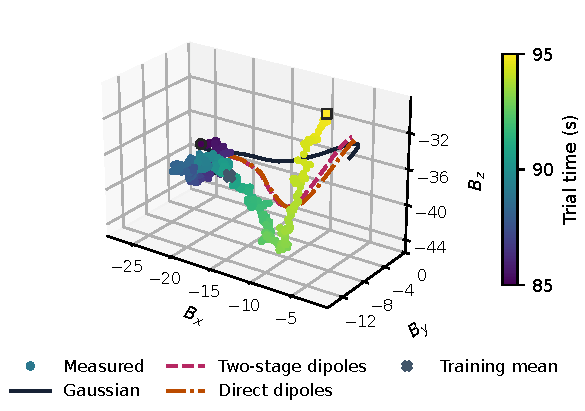
\includegraphics[width=\linewidth]{trial4_trajectory.pdf}
\end{minipage}\hfill
\begin{minipage}[c]{0.37\linewidth}
\caption{Magnetic vectors from 501 samples at 85--95 s, near the midpoint
of held-out Invensense trial 4. Color shows measurement time, from the
start circle to the end square. The lines evaluate the fitted models at
the same recorded positions. Axes show field components in reference
recording units.}
\label{fig:trajectory}
\end{minipage}
\end{figure}

Ten seconds of the held-out route make these errors visible in field space
(Figure~\ref{fig:trajectory}). As the robot moves, the tip of its magnetic
vector traces a three-dimensional curve. All three models follow the dip toward
lower \(B_z\) while underestimating its depth: the measured minimum reaches
\(-44.3\) units, compared with \(-41.4\) for the Gaussian map and \(-41.5\) to
\(-41.6\) for the two dipole maps. Along the route, the direct and two-stage
dipole curves lie almost on top of each other. To see what Gaussian smoothing
actually changed beneath that near-overlap, we can trace a single reading
through the fit.

\section{One field, two sums}

Equation~\eqref{eq:dipole_response} builds the dipole field from 100 assumed
sources. Once the measurement positions, source geometry, and penalties are
fixed, however, the fitted moments and background are linear functions of the
targets. That means the exact same predicted field can be rewritten as a
weighted sum over the 500 original readings.

Partition \(L\) in Eq.~\eqref{eq:ridge} into \(3M\times3\) block columns
\(L_a\) so that \(L\mathbf t=\sum_a L_a\mathbf t_a\). Substituting
\(\widehat{\mathbf q}\) and \(\widehat{\bvec}_0\) into
Eq.~\eqref{eq:dipole_response} expresses the dipole prediction directly in
terms of its targets:
\begin{equation}
 \widehat{\B}_D(\rr_*)=\bar{\mathbf t}+(D_*-\bar D)L\mathbf t
  =\sum_a U_a(\rr_*)\mathbf t_a,\qquad
 U_a(\rr_*)=\frac{I_3}{n}+(D_*-\bar D)L_a.
 \label{eq:direct}
\end{equation}
Each \(U_a(\rr_*)\) is a \(3\times3\) matrix giving the direct fit's weight on
raw reading \(a\). In the two-stage fit, each target is itself a Gaussian
average \(\mathbf t_a=\sum_i H_{ai}\bvec_i\); substituting this into
Eq.~\eqref{eq:direct} yields the two-stage measurement weights:
\begin{equation}
 \widehat{\B}_{\rm two}(\rr_*)=\sum_i W_i(\rr_*)\bvec_i,\qquad
 W_i(\rr_*)=\sum_a H_{ai}U_a(\rr_*).
 \label{eq:weights}
\end{equation}
Equating the source sum in Eq.~\eqref{eq:dipole_response} with the measurement
sum in Eq.~\eqref{eq:weights} gives the central identity
\begin{equation}
 \widehat{\B}_{\rm two}(\rr_*)=
 \widehat{\bvec}_0+\sum_{j=1}^{M}D(\rr_*,\mathbf s_j)\widehat{\mathbf q}_j
 =\sum_{i=1}^{n}W_i(\rr_*)\bvec_i .
 \label{eq:dipole_identity}
\end{equation}
The left-hand side tracks the superposition of physical dipole responses; the
right-hand side tracks each piece of empirical data into that exact same field.

This identity makes the effect of smoothing transparent. In the two-stage fit,
reading \(i\) feeds target \(a\) through the scalar \(H_{ai}\), and \(U_a\)
carries that target to the query, shifting reading \(i\)'s weight by
\(W_i-U_i=\sum_a(H_{ai}-\delta_{ai})U_a\) (where \(\delta_{ai}=1\) for \(a=i\)
and zero otherwise). At fixed positions and settings, perturbing reading \(i\)
by \(\Delta\) shifts the direct prediction by \(U_i\Delta\) and the two-stage
prediction by \(W_i\Delta\). Unlike the scalar weights \(g_{*i}\) of the
Gaussian map, the \(3\times3\) matrices \(U_i\) and \(W_i\) have off-diagonal
entries that carry perturbations from one measured component into another
predicted component. Meanwhile, both fits preserve any constant vector offset
because centering removes it from the moment fit and the background restores
it, giving \(\sum_i U_i=\sum_i W_i=I_3\).

Geomagnetic inversions use analogous linear weights to assess spatial
resolution and variance~\cite{hammer}. In machine learning, self-distillation
refits a model to its own predictions, which can both suppress noise and weaken
signal~\cite{mobahi,wu}. Our two-stage procedure distills once while changing
the model family from kernel to dipoles, and Eq.~\eqref{eq:weights} quantifies
the exact resulting shift in every reading's weight.

\subsection{The effect of one reading}

\begin{figure}[!htbp]
\centering
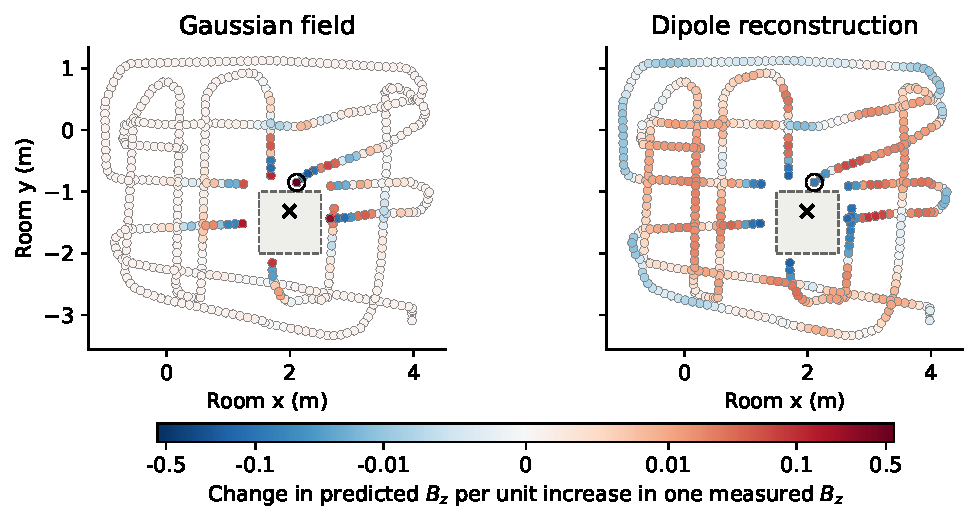
\includegraphics[width=.90\linewidth]{influence_map.pdf}
\caption{Effect of increasing one measured \(B_z\) by one unit on predicted
\(B_z\) at the cross. Dots mark training positions, the dashed box marks the
spatial gap, and a ring marks the reading with the largest absolute difference
in vertical weights between models at the query. The panels share a signed
color scale, linear within \(\pm 0.01\) and logarithmic beyond. Larger absolute
weights are drawn on top.}
\label{fig:influence}
\end{figure}

To see these weights in action, we select the held-out trial-4 position inside
the spatial gap nearest its center using coordinates alone:
\((1.990,-1.316)\) m, which lies \(0.482\) m from the nearest training reading.
Figure~\ref{fig:influence} compares the Gaussian weight \(g_{*i}\) against the
vertical-to-vertical entry \([W_i]_{zz}\) of the two-stage dipole weight across
all 500 training positions. The visual contrast is immediate: in the Gaussian
panel, influence concentrates tightly around the query cross, whereas in the
dipole panel, signed weights spread across the entire room.

The two maps diverge most sharply at the ringed reading \((2.109,-0.849)\) m,
just outside the gap. Raising that single reading's \(B_z\) by one unit pushes
predicted \(B_z\) \emph{up} by \(+0.579\) in the Gaussian map, but pushes it
\emph{down} by \(-0.025\) in the direct dipole fit and \(-0.085\) in the
two-stage dipole fit. Although a Gaussian kernel value is positive, its fitted
regression weights can have either sign. The reversal here is a property of
the complete regularized fits, not a consequence of kernel positivity. The
dipole basis enforces \(\nabla\cdot\B=0\) and \(\nabla\times\B=0\) above the
source plane while coupling components and distributing influence across
positions. Here, the direct dipole fit already flips the sign, and
pre-smoothing makes the response more than three times as negative, showing
that nearly identical route RMSEs can coexist with a substantial change in how
a specific reading is used. Across all three models, the analytical weights
match the archived query prediction and full refit perturbations in all three
components to within \(10^{-9}\) recording units.

The global reach of the physical model also appears in the weight distribution:
readings more than \(1\) m from the query carry \(33.0\%\) of the absolute
vertical weight in the Gaussian fit, but \(67.2\%\) in the two-stage dipole
fit. While both signed sums equal one, the sum of absolute vertical weights
nearly doubles from \(3.562\) to \(6.680\), reflecting stronger cancellation
between positive and negative weights. Cross-component coupling is likewise
substantial, with the largest absolute weight from a horizontal reading to
predicted \(B_z\) reaching \(0.469\) in the two-stage fit.

\section{Hiding the law in a wire experiment}

Return to the compass beside a current. In the room, we handed the learner the
dipole response before fitting its coefficients. With a simulated wire, we can
remove that crutch and ask the learner to choose the mathematical form itself,
while fixing the geometry and varying the current so that the exact field
provides a clean ground truth.

For a steady signed current \(I\) along the \(z\) axis of an ideal infinite
wire, Amp\`ere's law gives \(\oint\B\cdot d\boldsymbol\ell=\mu_0 I\), where
\(d\boldsymbol\ell\) is the oriented line element. By cylindrical symmetry, the
field is tangent to circles of radius \(r=\sqrt{x^2+y^2}\) with signed
tangential magnitude \(B_\varphi=\mu_0 I/(2\pi r)\) and unit tangent
\((-y,x,0)^{\mathsf T}/r\). In microtesla, with \(x,y\) in metres and \(I\) in
amperes, the simulator evaluates
\begin{equation}
 \B_*(x,y,I)=0.2I\frac{(-y,x,0)^{\mathsf T}}{x^2+y^2}.
 \label{eq:wire_truth}
\end{equation}
The learner observes sampled inputs \(\mathbf u=(x,y,I)\) paired with noisy
field readings; for kernel fitting, the three inputs are standardized on the
training set.

Both the two-stage and direct routes search the same candidate library:
polynomial fields through degree 4 and rational fields of degree 1 or 2. Each
rational candidate takes the form \(p_c(\mathbf u)/q(\mathbf u)\) for
components \(c=1,2,3\), sharing a polynomial denominator \(q\) with separate
polynomial numerators \(p_c\). Given target \(t_{ic}\) at input \(\mathbf u_i\),
we initialize by solving \(t_{ic}q(\mathbf u_i)-p_c(\mathbf u_i)\approx0\) via
homogeneous least squares, prune small coefficients, fix the denominator scale,
and refit to the field values by nonlinear least squares. As before, the
two-stage route fits to Gaussian kernel predictions whereas the direct route
fits to raw readings. Each route selects the sparsest candidate within \(5\%\)
of its lowest validation mean squared error (plus a numerical tolerance), and
both are scored against the exact field on independent test points.

Gaussian process smoothing is often used to denoise data before symbolic
regression~\cite{hsin}, while input ranges~\cite{matsubara} and
complexity--accuracy trade-offs~\cite{fong} strongly affect which expressions
are recovered. Holding the search space and selection rule fixed isolates the
effect of pre-smoothing.

\begin{table}[!htbp]
\centering
\caption{Hidden-wire error on independent inputs in each training domain.
For each seed, vector RMSE is divided by the root mean square of the true field
magnitudes. Entries are percentages averaged over three seeds; the noiseless
direct error rounds to zero.}
\label{tab:wire}
\small
\begin{tabular}{@{}lrrr@{}}
\toprule
Case & Gaussian & Two-stage expression & Direct expression\\
\midrule
Noiseless                & 20.42 & 0.35 & 0.00 \\
Main, \(1\%\) noise      & 20.44 & 0.38 & 0.06 \\
Higher noise, \(5\%\)    & 21.18 & 0.60 & 0.28 \\
Sparse, \(1\%\) noise    & 51.10 & 6.23 & 0.10 \\
Limited angles, \(1\%\)  &  3.62 & 0.16 & 0.04 \\
\bottomrule
\end{tabular}
\end{table}

The main case uses 480 training and 180 validation readings across radii
\(0.25\)--\(2\) m, all angles, and currents \(|I|=0.5\)--\(4\) A, corrupted by
independent Gaussian noise at \(1\%\) of the pooled RMS of the clean training
components. The sparse regime cuts training to 80 readings, and limited angles
restrict azimuth to \(\pm\pi/6\) radians; every test domain uses 800 fresh
points.

\begin{samepage}
All 15 two-stage fits (five cases across three seeds) select the exact same
monomials. Here is the generating field beside the reconstruction from the
first seed in the main case, with fitted coefficients rounded for display:
\[
\begin{array}{c@{\qquad}c}
\text{Generating field} & \text{Field recovered through the kernel}\\[4pt]
\displaystyle\frac{0.2 I}{x^2+y^2}
  \begin{pmatrix}-y\\x\\0\end{pmatrix}
&
\displaystyle\frac{I}{1.003060 x^2+y^2}
  \begin{pmatrix}-0.198992 y\\0.199601 x\\0\end{pmatrix}.
\end{array}
\]
\par
\end{samepage}
\begin{samepage}
Normalizing the \(y^2\) coefficient to one puts every recovered expression in
the form \(I(-a y,b x,0)^{\mathsf T}/(c x^2+y^2)\). Two physical symmetries
follow exactly from that form: doubling the current doubles the field, and
doubling both coordinates at fixed current halves it. Circular symmetry, which
also requires \(a=b\) and \(c=1\), holds approximately.
\par
\end{samepage}

In the main case, fitting a rational expression to the Gaussian map slashes the
error from \(20.44\%\) down to \(0.38\%\), and that accuracy holds when
extrapolating to larger radii (\(0.38\%\)) and unseen currents (\(0.38\%\)).
Yet direct fitting on the raw readings does better in every single row of
Table~\ref{tab:wire}, dropping the main-case error to \(0.06\%\) and the
sparse-data error from \(6.23\%\) to \(0.10\%\). The reason is clear in the
first column of Table~\ref{tab:wire}: even when the Gaussian kernel selects the
shortest length scale tested, it struggles to track the rapid \(1/r\) variation
near the wire, especially with only 80 readings (\(51.10\%\) error). Because
the candidate library already contains the true rational family, fitting
directly to the raw measurements avoids inheriting the smoother's bias.

Finally, the wire illustrates a hard limit on what measurements can determine
when a controlling variable goes unrecorded. At any fixed position, the field
is proportional to the signed current; if positive and negative currents occur
with equal probability at each position and magnitude, the conditional mean
given position alone is zero. Under squared error, zero is the best prediction
any position-only model can make, a reminder that even the right
equation cannot overcome an unobserved source, whether a hidden current or
unmapped shelves in a room.

\section{What the readings determine}

Both experiments trace the path from raw measurements to an equation that can
be evaluated at new inputs. In the indoor room, choosing the physical dipole
form accounts for almost all of the gain over a Gaussian map, while
pre-smoothing barely alters route error. In the wire experiment, where the
learner must also choose the terms of the law, direct fitting on raw readings
outperforms pre-smoothing in every regime we tested.
The added tree baselines also trail the dipoles on the measured room, although
their model classes and tuning budgets differ.

\begin{samepage}
The indoor experiment also makes visible how empirical data enter a textbook
field. Collecting Eqs.~\eqref{eq:gaussian_response}, \eqref{eq:teacher}, and
\eqref{eq:dipole_identity} places the three models side by side. Superscripts
\(d\) and \(s\) mark coefficients fitted to raw and smoothed targets, and we
write \(k_{*i}=k_\ell(\x_*,\x_i)\) and \(D_{*j}=D(\rr_*,\mathbf s_j)\):
\[
\begin{array}{lccc}
 & \text{Sum of fitted responses} && \text{Sum over training readings}\\[3pt]
\text{Gaussian} &
\displaystyle\overline{\B}+\sum_i k_{*i}\boldsymbol\alpha_i
&=& \displaystyle\sum_i g_{*i}\bvec_i\\[7pt]
\text{Direct dipoles} &
\displaystyle\widehat{\bvec}_0^d+\sum_j D_{*j}\widehat{\mathbf q}_j^d
&=& \displaystyle\sum_i U_i(\rr_*)\bvec_i\\[7pt]
\text{Two-stage dipoles} &
\displaystyle\widehat{\bvec}_0^s+\sum_j D_{*j}\widehat{\mathbf q}_j^s
&=& \displaystyle\sum_i W_i(\rr_*)\bvec_i .
\end{array}
\]
\par
\end{samepage}
Each dipole row writes one field in two equivalent ways: as a sum over 100
assumed sources (\(j\)) or as a sum over 500 actual readings (\(i\)). Classical
theory supplies the response matrix \(D_{*j}\) of each source, while the
observations determine the fitted moments and background. Reading the right-hand
side tells us the exact change in any prediction when a single sensor value
shifts, a precise sense in which a field with a textbook form learns from
examples.

Three claims should be kept separate. The dipole basis satisfies the assumed
static equations away from its sources; the source and measurement sums are
exactly equivalent evaluations of one fitted field; and held-out RMSE measures
how well that field predicts observations. Neither equation compliance nor an
exact rewrite guarantees predictive accuracy. A companion traveling-wave
study~\cite{stumps} makes the distinction explicit: phase-based stumps and a
phase-based forest both give exact weak Maxwell solutions, yet the forest fits
the tested pulse more accurately. The propagation law and field coupling are
supplied there, just as magnetostatics is supplied by the dipole basis here.

\paragraph{Scope and limitations.}
These conclusions describe the specific estimators and domains tested here. The
indoor comparison covers one room and previously examined trials, and trial 3
selected the shared dipole settings for the two-stage fit; a comparison of
fully tuned procedures would tune the direct fit separately, and a
scalar-potential Gaussian process offers another physics-based
baseline~\cite{solin}. Moreover, both grid size and depth reached the upper
limits of our search, planar measurements leave three-dimensional sources
underdetermined, and route-based scores measure accuracy along robot paths
rather than uniformly across the room~\cite{wadoux}.

\paragraph{Data and code.}
The \href{https://github.com/AaltoML/magnetic-data/tree/b45da3bc7ab623fdef6e01247021daebf7983f29}{Aalto recordings}
are pinned to commit \texttt{b45da3b}. The
\href{https://github.com/jonland82/blind-field-discovery/tree/52cd50c}{project repository}
contains the companion notes, code, fixed protocols, saved predictions,
and fitted dipole coefficients.
The additional baselines and complete validation grids are retained in the
\href{https://github.com/jonland82/blind-field-discovery/tree/52cd50c/experiments/magnetic_mapping/tree_comparison}{tree-comparison directory}.

\clearpage
\appendix
\section{A scalar check with a known differential law}
\label{sec:scalar}

To check how these ideas carry over to a differential law, we test a scalar
system with known dimensionless field \(B_*(x)=1.7\tanh(x/0.9)\) and source
\(J_*(x)=0.8\sech^2(x/0.9)\), where \(\sech u=1/\cosh u\). Both channels are
sampled at 80 positions with noise at \(0.1\%\) of each channel's amplitude,
and Gaussian models are fitted to each. Differentiating the fitted field
\(\widehat B\) supplies targets for sparse regression: with both \(B\) and
\(J\) available, the search selects \(B'=aJ\) (prime denoting \(d/dx\)),
recovering \(a_*=1.7/(0.9\cdot0.8)=85/36\) to \(0.022\%\) relative error.
Integrating from the boundary value \(b_0\) at \(x_0=-3\) yields
\(b_0+a\int_{x_0}^x\widehat J(u)\,du\).

Restricting the search to powers of \(B\) alone selects \(B'=p-qB^2\) with
\(p,q>0\). Separating variables on \(|B|<A\) gives the closed-form solution
\[
 B(x)=A\tanh((x-x_c)/L),\qquad J(x)=(p/a)\sech^2((x-x_c)/L),
 \qquad A=\sqrt{p/q},\quad L=1/\sqrt{pq},
\]
with center \(x_c\) fixed by the fitted field at the median training position.
On the noisy test grid, relative Euclidean errors are \(0.045\%\) for the
solved field, \(0.085\%\) for the Gaussian fit, and \(0.229\%\) for the
integral reconstruction. Both reconstructions use the recovered channel
relation, but only the field-only equation also recovers the analytic shape of
the generating function.

{\small
\begin{thebibliography}{99}
\bibitem{maxwell}
J.~C. Maxwell.
A dynamical theory of the electromagnetic field.
\emph{Philosophical Transactions of the Royal Society of London}, 155:459--512, 1865.
\href{https://doi.org/10.1098/rstl.1865.0008}{doi:10.1098/rstl.1865.0008}.

\bibitem{solin}
A. Solin, M. Kok, N. Wahlstr\"om, T.~B. Sch\"on, and S. S\"arkk\"a.
Modeling and interpolation of the ambient magnetic field by Gaussian processes.
\emph{IEEE Transactions on Robotics}, 34(4):1112--1127, 2018.
\href{https://doi.org/10.1109/TRO.2018.2830326}{doi:10.1109/TRO.2018.2830326}.

\bibitem{chang}
P.~E. Chang, P. Verma, S.~T. John, A. Solin, and M.~E. Khan.
Memory-based dual Gaussian processes for sequential learning.
\emph{Proceedings of the 40th International Conference on Machine Learning},
PMLR 202:4035--4054, 2023.
\href{https://proceedings.mlr.press/v202/chang23a.html}{Proceedings}.

\bibitem{abdulraouf}
I. Abdul-Raouf, V. Gay-Bellile, C. Joly, S. Bourgeois, and A. Paljic.
Large scale mapping of indoor magnetic field by local and sparse Gaussian
processes.
\emph{Proceedings of the 8th Conference on Robot Learning},
PMLR 270:2104--2119, 2025.
\href{https://proceedings.mlr.press/v270/abdul-raouf25a.html}{Proceedings}.

\bibitem{emilia}
D.~A. Emilia.
Equivalent sources used as an analytic base for processing total magnetic
field profiles.
\emph{Geophysics}, 38(2):339--348, 1973.
\href{https://doi.org/10.1190/1.1440344}{doi:10.1190/1.1440344}.

\bibitem{uppal}
I. Uppal and R. Holme.
Dual-layer gradient-boosted equivalent sources for magnetic data.
\emph{Geophysical Journal International}, 243(3):ggaf359, 2025.
\href{https://doi.org/10.1093/gji/ggaf359}{doi:10.1093/gji/ggaf359}.

\bibitem{hammer}
M.~D. Hammer and C.~C. Finlay.
Local averages of the core--mantle boundary magnetic field from satellite observations.
\emph{Geophysical Journal International}, 216(3):1901--1918, 2019.
\href{https://doi.org/10.1093/gji/ggy515}{doi:10.1093/gji/ggy515}.

\bibitem{mobahi}
H. Mobahi, M. Farajtabar, and P.~L. Bartlett.
Self-distillation amplifies regularization in Hilbert space.
\emph{Advances in Neural Information Processing Systems}, 33, 2020.
\href{https://proceedings.neurips.cc/paper/2020/hash/2288f691b58edecadcc9a8691762b4fd-Abstract.html}{Proceedings}.

\bibitem{wu}
M. Wu, A.~Y. Yang, and Q. Sun.
Why self-distillation helps and hurts: Denoising vs. signal forgetting.
\emph{Proceedings of the 43rd International Conference on Machine Learning},
PMLR 306:137334--137367, 2026.
\href{https://proceedings.mlr.press/v306/wu26bs.html}{Proceedings}.

\bibitem{hsin}
J. Hsin, S. Agarwal, A. Thorpe, L. Sentis, and D. Fridovich-Keil.
Symbolic regression on sparse and noisy data with Gaussian processes.
\href{https://arxiv.org/abs/2309.11076}{arXiv:2309.11076}, 2024.

\bibitem{matsubara}
Y. Matsubara, N. Chiba, R. Igarashi, and Y. Ushiku.
Rethinking symbolic regression datasets and benchmarks for scientific discovery.
\emph{Journal of Data-centric Machine Learning Research}, 2024.
\href{https://data.mlr.press/assets/pdf/v01-3.pdf}{Article}.

\bibitem{fong}
K.~S. Fong and M. Motani.
Pareto-optimal fronts for benchmarking symbolic regression algorithms.
\emph{Proceedings of the 42nd International Conference on Machine Learning},
PMLR 267:17392--17410, 2025.
\href{https://proceedings.mlr.press/v267/fong25b.html}{Proceedings}.

\bibitem{wadoux}
A.~M.~J.-C. Wadoux, G.~B.~M. Heuvelink, S. de Bruin, and D.~J. Brus.
Spatial cross-validation is not the right way to evaluate map accuracy.
\emph{Ecological Modelling}, 457:109692, 2021.
\href{https://doi.org/10.1016/j.ecolmodel.2021.109692}{doi:10.1016/j.ecolmodel.2021.109692}.
\bibitem{stumps}
J.~R. Landers.
Decision stumps as exact Maxwell fronts.
Companion research note, 2026.
\href{https://github.com/jonland82/blind-field-discovery/blob/52cd50c/papers/05-equivalent-descriptions/stumps_as_maxwell_fronts.pdf}{Companion paper}.

\end{thebibliography}}
\end{document}
